%!TEX root = ../../main.tex

\chapter{Anleitung für Dozierende}
\label{sec:chap2}

\section{Kursübersicht}
Meldet sich ein Dozent bei eCourse an, wird er direkt auf die Kursübersicht geleitet. Auf diese Ansicht kann der Nutzer zu jedem Zeitpunkt zurückkehren, indem er in der Menüleiste den Punkt \glqq Kursübersicht \grqq{} auswählt. In der Kursübersicht werden dem Nutzer alle Kurse angezeigt, in denen er Mitglied ist. Eine beispielhafte Kursübersicht ist in Abbildung \ref{fib:kursübersicht_dozent} gezeigt.

\begin{figure}[h]
\centering
\includegraphics[width=0.9\textwidth]{kursübersicht_dozent.png}
\caption{Kursübersicht eines Dozenten in der Anwendung eCourse}
\label{fib:kursübersicht_dozent}
\end{figure}

Möchte der Dozent mehr Informationen zu einem bestimmten Kurs erhalten, erhält er diese, indem er den Kurs in der Kursübersicht ausklappt. Dann werden ihm alle Mitglieder des bestimmten Kurses angezeigt und auch alle Aufgaben, die er dem Kurs gestellt hat. Beispielhaft ist dies in Abbildung \ref{fib:kursübersicht_dozent_ausgeklappt} gezeigt. Genauere Details zu einer Aufgabe erhält der Dozent, indem er in der ausgeklappten Kursübersicht auf die Schaltfläche \glqq anzeigen\grqq{} neben der gewünschten Aufgabe klickt. Genauere Informationen finden sich in Kapitel \ref{sec:herunterladen}. Möchte der Dozent die Aufgabe bearbeiten erreicht er dies indem er auf die Schaltfläche \glqq Bearbeiten\grqq{} klickt. Genauere Informationen dazu finden sich in Kapitel \ref{sec:bearbeiten}
 
\begin{figure}[h]
\centering
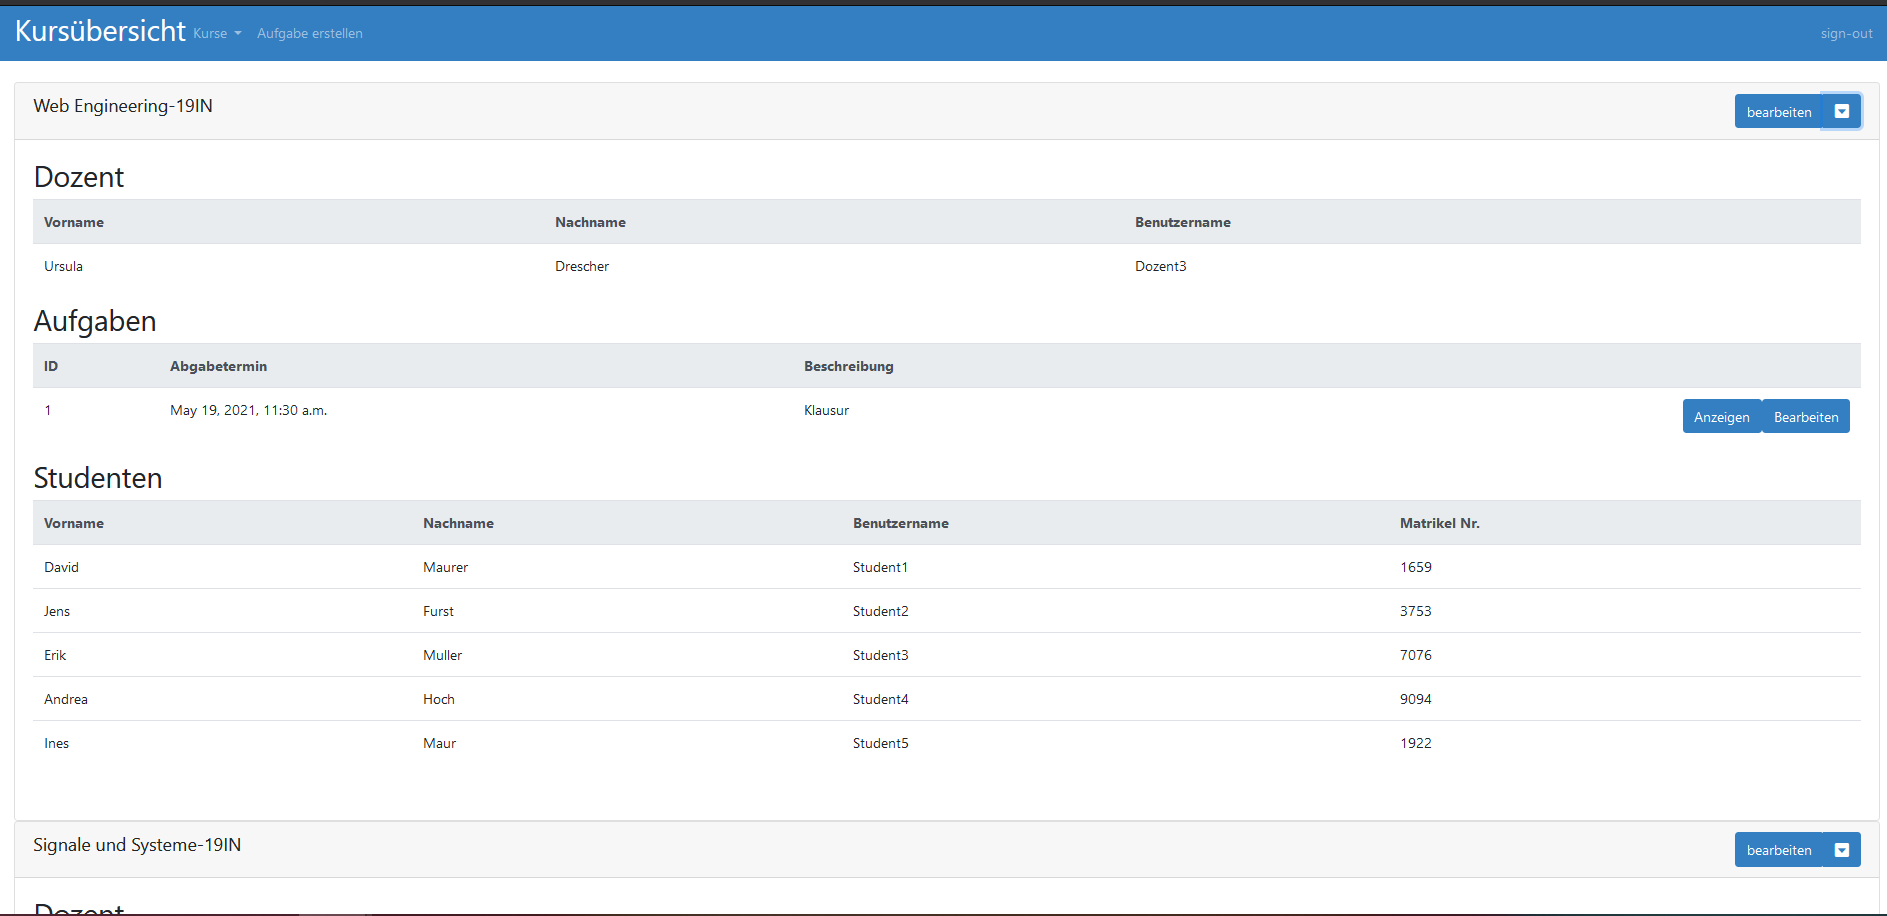
\includegraphics[width=0.9\textwidth]{kurse_ausgeklappt_dozent.png}
\caption{Ausgeklappte Kursübersicht eines Dozenten in der Anwendung eCourse}
\label{fib:kursübersicht_dozent_ausgeklappt}
\end{figure}

\section{Kurs erstellen}
Möchte der Dozent selbst einen Kurs erstellen, kann er dies, indem er in der Menüleiste den Unterpunkt \glqq Kurs erstellen\grqq{} auswählt. Dadurch gelangt er auf eine Unterseite mit dem entsprechenden Formular um einen Kurs anzulegen. Das Formular ist in Abbildung \ref{fib:kurs_anlegen} gezeigt. Alle Felder des Formulars müssen ausgefüllt sein. Aus der Liste der Dozenten muss der Dozent sich selbst als Dozent des Kurses auswählen.
Die Teilnehmer am Kurs aus der Gruppe der Studierenden werden hinzugefügt, indem man sie anhand ihres Benutzernamens in der Liste ausfindig macht und mit einem Haken versieht. \\
Außerdem sollte dem Kurs sinnvoller Name vergeben werden. Von den Entwicklern wird ein Name empfohlen der dem folgenden Schema entspricht: \\
\verb/Kursname_JJKursbezeichnung/\\
Abschließend kann über einen Kalender ein Start- und Enddatum des Kurses festgelegt werden. 
Die Erstellung des Kurses kann durch klicken der Schaltfläche \glqq Kurs erstellen\grqq{} beendet werden.

\begin{figure}[h]
\centering
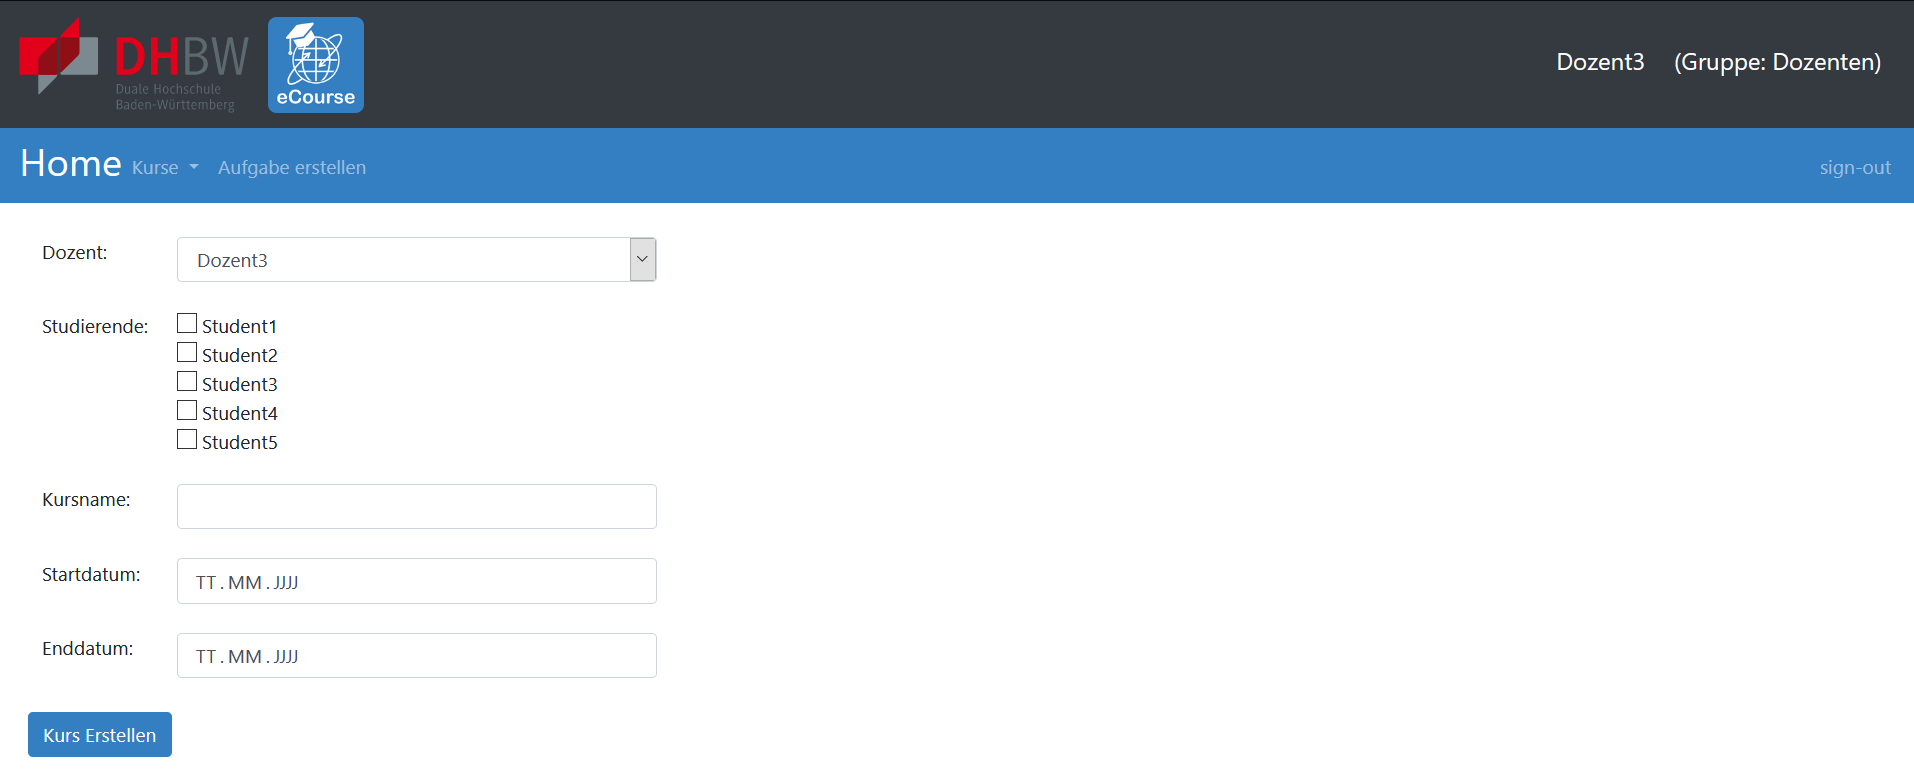
\includegraphics[width=0.9\textwidth]{kurs_erstellen_dozent.png}
\caption{Kurs Anlegen durch einen Dozenten in der Anwendung eCourse}
\label{fib:kurs_anlegen}
\end{figure}
\section{Kurs bearbeiten}
Kurse können nur bearbeitet werden, wenn sich der Benutzer in der Kursübersicht befindet. Dort findet sich neben jedem Kursnamen eine Schaltfläche \glqq bearbeiten\grqq . Wird diese betätigt öffnet sich das gleiche Formular wie auch bei der Kurserstellung. Im Gegensatz zum Anlegen des Kurses ist das Formular aber hier mit den Informationen über den Kurs gefüllt und kann bei Bedarf abgeändert werden.\\
Wurden Änderungen vorgenommen, werden diese gespeichert in dem der Nutzer die Schaltfläche \glqq Speichern\grqq{} betätigt.\\
Möchte der Benutzer keine Änderungen vornehmen, kann er über die Schaltfläche \glqq zurück\grqq{} zurück auf die Kursübersicht gelangen.


\section{Aufgabe erstellen}
Möchte der Dozent den Mitgliedern eines Kurses eine Aufgabe stellen, kann er dies tun, indem er eine Aufgabe erstellt. Dazu kann in der Menüleiste der Punkt \glqq Aufgabe erstellen\grqq\; ausgewählt werden. Dadurch öffnet sich sich ein Formular (siehe Abbildung \ref{fib:aufgabe_anlegen}). 
In diesem Formular muss der entsprechende Kurs ausgewählt werden für den eine Aufgabe erstellt werden soll. Außerdem muss für die Aufgabe eine Startzeit und eine Endzeit festgelegt werden. Diese beiden Zeiten definieren den Beginn und das Ende der Zeitspanne in der die Mitglieder des Kurses Dateien zu der Aufgabe hochladen können. \\
Außerdem muss das Feld der Bearbeitungszeit ausgefüllt werden. Hier wird angegeben wie lange die Mitglieder Zeit haben die Aufgabe zu bearbeiten. Dabei sollte beachtet werden, dass den Mitgliedern zusätzliche Zeit eingeräumt werden sollte, um die Lösungen hochzuladen.\\
Abschließend muss noch eine Beschreibung der Aufgabe hinzugefügt werden. 
Die Schaltflächen \glqq sichtbar\grqq{} und \glqq benotet\grqq{} sind optionale Parameter.

\begin{figure}[h]
\centering
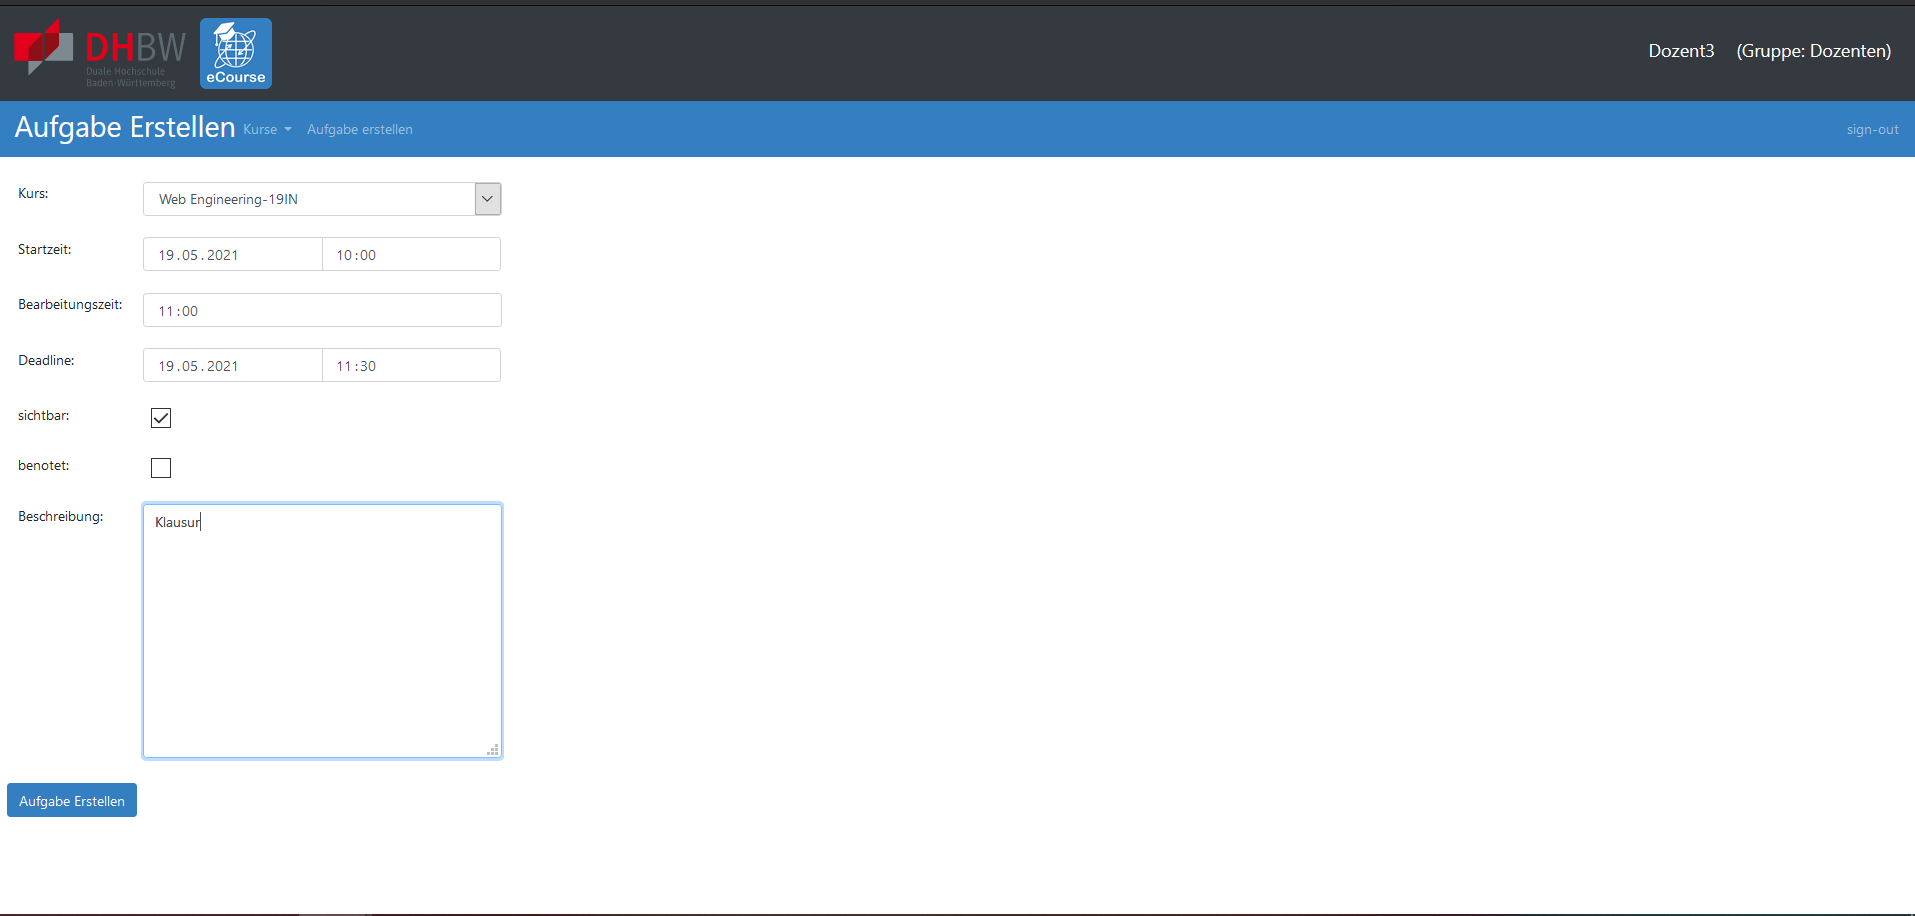
\includegraphics[width=0.9\textwidth]{aufgabe_erstellen_dozent.png}
\caption{Aufgabe erstellen in der Anwendung eCourse}
\label{fib:aufgabe_anlegen}
\end{figure}


\section{Aufgabe bearbeiten}
\label{sec:bearbeiten}
Der Dozent kann die Aufgabe bearbeiten indem er in der ausgeklappten Kursübersicht die Schaltfläche \glqq Bearbeiten\grqq{} betätigt. Dadurch öffnet sich eine ähnliche Ansicht als würde eine Aufgabe erstellt werden. Allerdings ist hier das Formular bereits ausgefüllt (siehe Abbildung \ref{fib:aufgabe_bearbeiten} ).\\
Hier können Aufgaben sowohl bearbeitet werden, als auch gelöscht. 
Dies sollte unter größter Sorgfalt geschehen, da die Betätigung der Schaltfläche \glqq Löschen\grqq{} zum sofortigen Löschen des Kurses führt. Die Löschung eines Kurses wird durch das Anzeigen einer Erfolgsmeldung bestätigt. Über betätigen der dort angezeigten \glqq zurück\grqq{} Schaltfläche gelangt der Nutzer wieder zurück auf die Kursübersicht.

\begin{figure}[h]
\centering
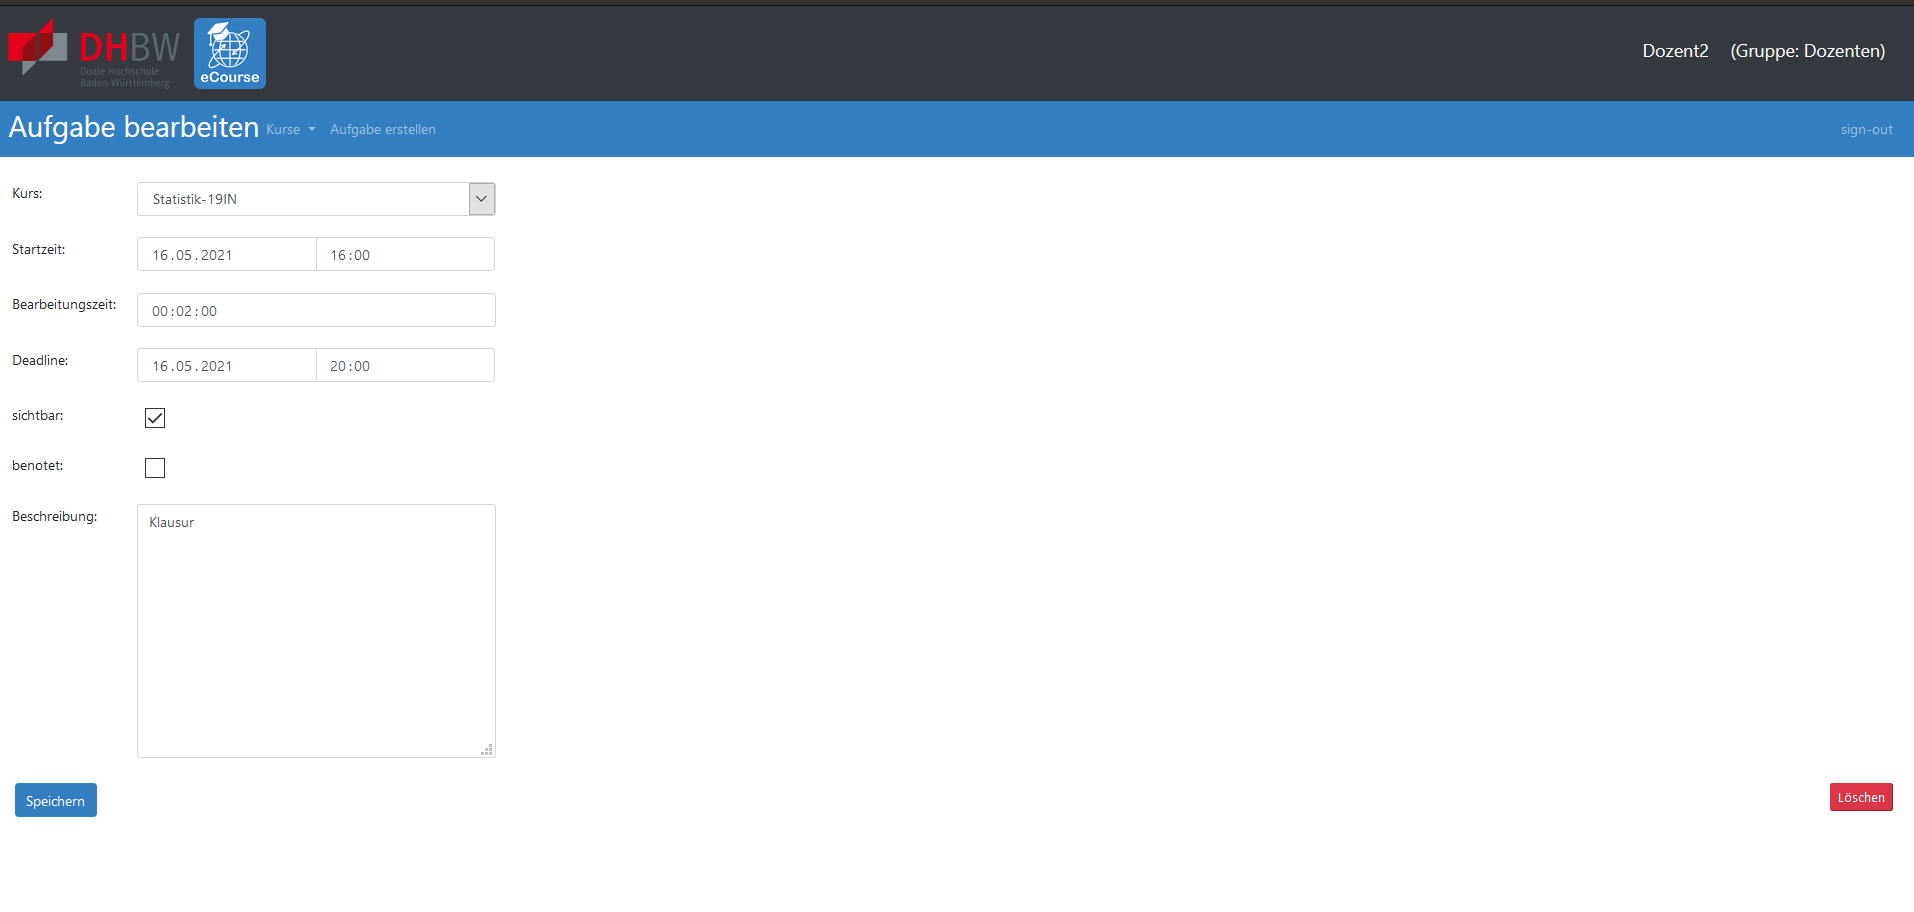
\includegraphics[width=0.9\textwidth]{aufgabe_bearbeiten.png}
\caption{Aufgabe bearbeiten in der Anwendung eCourse}
\label{fib:aufgabe_bearbeiten}
\end{figure}

\section{Bearbeite Abgaben herunterladen}
\label{sec:herunterladen}
Möchte der Dozent die Abgaben der Mitglieder seines Kurses einsehen, kann er dies, indem er von der ausgeklappten Kursübersicht aus die Schaltfläche \glqq anzeigen\grqq{} auswählt. Dadurch wird ihm eine Seite wie in Abbildung \ref{fib:aufgabe_bearbeiten} gezeigt. Von dort kann er die Abgaben der Mitglieder herunterladen un dadurch einsehen. Außerdem kann er weitere Dateien hochladen.

\begin{figure}[h]
\centering
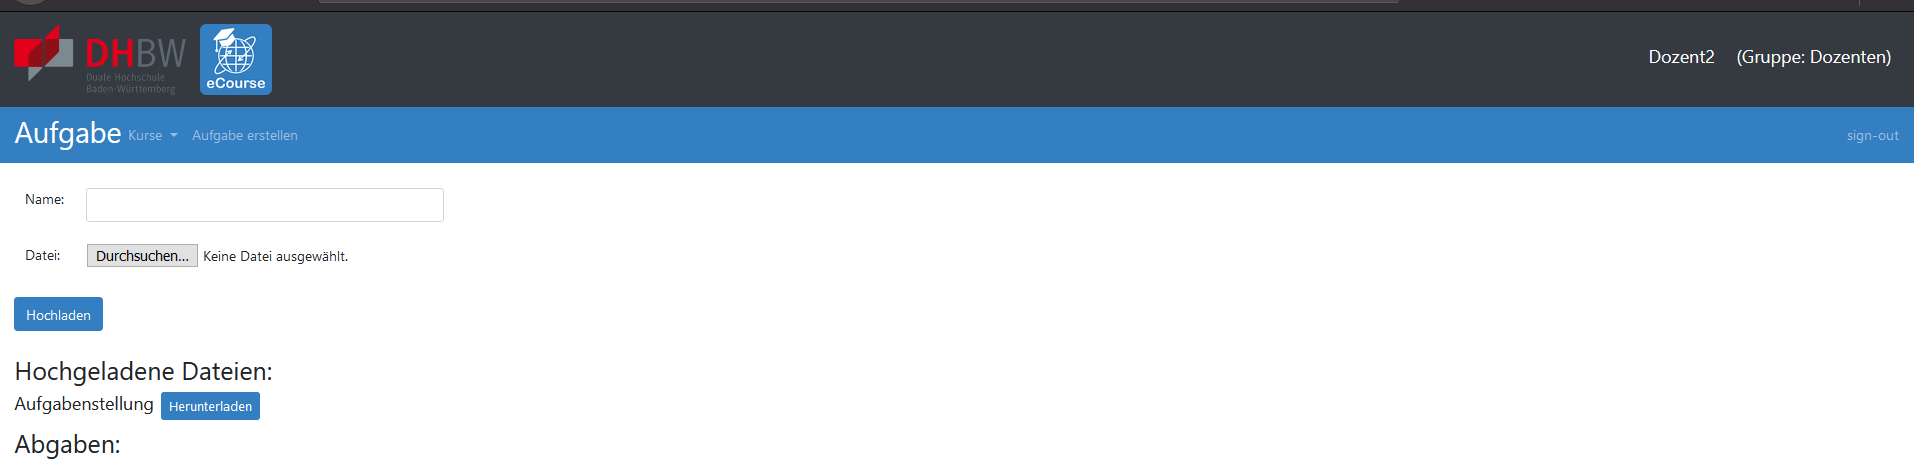
\includegraphics[width=0.9\textwidth]{aufgabe_bearbeiten_dozent.png}
\caption{Abgaben anzeigen in der Anwendung eCourse}
\label{fib:aufgabe_bearbeiten}
\end{figure}
